\section{Heurística Constructiva Golosa}
\subsection{Implementación del Algoritmo}

\par{La heurística golosa consiste en construír una solución por partes. El
algoritmo itera y en cada iteración agrega una parte a la solución. Sea $S$
una solución a un problema dado, llamamos $S_i$ a una subsolución de $S$, es
decir una solución incompleta al problema. Sea $S_i$ = $\{s_1, s_2\dots s_i\}$
la subsolución obtenida en la iteración $i$ de la heurística, y sea $P_i$ =
$\{p_1, p_2\dots p_n\}$ el conjunto de posibles $partes$ de solución tales que
$S_i \cup p_j$ sea también subsolución del problema. Entonces $P_i$ es el
conjunto de candidatos de la iteración $i$. En la iteración $i$, la heurística
golosa debe $elegir$ entre un conjunto $P_i$ de candidatos y una vez
seleccionado el $p_j$ del conjunto, generar una subsolución $S_{i+1}$ compuesta
por $S_i$ y $p_j$. La forma en que se elige el $p_j$ es mediante una función
que le asigna a cada $p_j$ (o a cada $S_i \cup p_j$) un valor numérico. La
heurística golosa elegirá a aquel $p_j$ que maximice dicha función.}\\

\par{En el problema de $CMF$ una solución es un conjunto de nodos. Así que la
heurística golosa implementada construirá el conjunto de nodos solución
agregando un nodo en cada iteración. La función que utilizamos para
seleccionar al mejor candidato (el nodo a agregar) es cuánto incrementaría la
frontera de la solución si se agreagra ese nodo a la solución parcial. Cuando
ningún nodo ampliaría la frontera de la solución parcial (o cuando ya no quedan
nodos que agregar) el algoritmo termina y retorna la solución almacenada. A
continuación se presenta un pseudocódigo de la solución implementada.}\\

\begin{algorithm}[H]
	\caption{Pseudocódigo de la heurística constructiva golosa}
	\KwData{\textbf{Grafo} $G(V,E)$}
	\textbf{Solucion} $solucion\_actual$ $\leftarrow$ $solucion\_vacia$\\
	\While{Puedo agregar nodos}{
		\textbf{int} $candidato$ $\leftarrow$ -1\\
		\textbf{int} $maximo\_aporte$ $\leftarrow$ 0\\
		\For{( \textbf{int} $nodo$ $\in$ $V$, $nodo$ $\notin$ $solucion\_actual$) )}{
			\If{$se\_conecta\_con\_clique$($i$, $solucion\_actual$)}{
				\textbf{int} $aporta$ $\leftarrow$ $cuanto\_aporta(nodo,\ solucion\_actual)$\\
				\If{$aporta >\ maximo\_aporte$}{
					$candidato$ $\leftarrow$ $nodo$\\
					$maximo\_aporte$ $\leftarrow$ $aporta$
				}
			}
		}
		\eIf{$candidato$ = -1}{
			Ya no puedo agregar nodos\\
		}{
			Agregar $candidato$ a $solucion\_actual$\\
		}
	}
	\textbf{return} $solucion\_actual$
\end{algorithm}

\par{Una vez más se inicia con una solución vacía (un conjunto de nodos
vacío). Cualquier nodo con al menos una arista va a sumar a la frontera si
se lo agrega a la solución, por lo que, una vez más el algoritmo devuelve el
conjunto vacío sólo si el grafo no tiene aristas. En cada iteración se
le asigna -1 a la variable $candidato$ la cual contendrá el nodo candidato
a ser agregado a la solución. Luego se itera sobre todos los nodos del grafo
y para cada uno se evalúa cuánto incrementaría la frontera de la solución si
se lo agregara a ella. Si luego de recorrer todos los nodos $candidato$ sigue
valiendo -1, significa que o bien ya todos los nodos están en la solución,
o bien ningún nodo que puede ser agregado aumentaría la frontera de la
solución. Si es ese el caso, se deja de iterar el ciclo principal (línea 2
del pseudocódigo) y se devuelve la $solucion\_actual$.}\\

\par{Luego de iterar sobre todos los nodos, si $candidato$ no vale -1, se
agrega el nodo $candidato$ a la $solucion\_actual$. La función
$se\_conecta\_con\_clique$ retorna si al agregar determinado nodo a una
solución, esta sigue siendo una clique. La función $cuanto\_aporta$
determina cuanto incrementaría (o decrementaría) la frontera de una
solución al agregarle un determinado nodo. Tras iterar sobre todos los
nodos $candidato$ almacena el nodo que más incrementaría el tamaño de la
frontera de la $solucion\_actual$.}

\subsection{Orden de complejidad}

\par{El ciclo prinicipal no puede iterar más de $n$ veces, ya que no se pueden
agreagar más de $n$ nodos a un conjunto de nodos que es subconjunto de los
nodos del grafo. En cada iteración del ciclo principal se recorren todos los
nodos del grafo y, para cada nodo que no pertenece al conjunto se evalúa
cuánto aportaría agregarlo. Dado que el conjunto se representa con un
arreglo de booleanos, ver si el i-ésimo nodo pertenece al conjunto consiste
en evaluar el i-ésimo booleano del arreglo, lo cual se hace en orden constante.
La función $se\_conecta\_con\_clique$\footnote{Tanto esta función como la que
agrega nodos a la solución son las mismas que las utilizadas en el algoritmo
exacto, son funciones declaradas en la clase $grafo$.} tiene complejidad
lineal en la cantidad de nodos del conjunto, la cual puede acotarse
superiormente por $n$.}\\

\par{La función $cuanto\_aporta$, también de la clase $grafo$, calcula
cuánto incrementaría la frontera de la solución agregándole el nodo y
recalculando la frontera de la solución. Hemos visto ya que agregar o quitar
nodos tiene complejidad lineal en el grado del nodo agregado o quitado, el
cual también puede ser acotado superiormente por la cantidad de nodos del
grafo. Finalmente, la complejidad de la heurística constructiva golosa es
$n * ((n * (n+n)) + n) \in$ O($n^3$).}

\subsection{Comportamiento}

\par{En la primera iteración, la heurística agrega a la solución el nodo
de mayor grado. Dado que se parte del conjunto vacío, cualquier nodo
puede ser agregado a la solución y formará una clique de un nodo, en el
que la frontera sea la cantidad de aristas que inciden sobre el nodo. Con
esto podemos afirmar que la heurística golosa encuentra la solución óptima
en grafos estrella\footnote{Un grafo con un nodo central y el resto de los
nodos unidos únicamente al nodo central, es decir un bipartito $K_{1n}$} o
en grafos cuyas componentes conexas son todas estrellas.}\\

\par{Esto también nos da una cota inferior al resultado devuelto por la
heurística. Dado que, una vez obtenida una solución, sólo se agregan nodos
si hacerlo mejora la solución, entonces la heurística golosa nunca devolverá
una solución con frontera menor al grado máximo del grafo. Sin embargo, esto
no nos dice que tan cerca puede estar de la solución óptima, ya que la frontera
de la $CMF$ puede ser tanto mayor al grado máximo como uno quiera.}\\

\par{Por ejemplo, un grafo $G$ con una componente conexa que es una estrella
de $\Delta$($G$)+1 nodos (con $\Delta$($G$) el grado máximo del grafo $G$) y
otra componente conexa de dos nodos adyacentes, cada uno adyacente a
otros $\Delta$($G$)-2 nodos. La heurística tomaría como primer nodo el centro
de la estrella que es adyacente a $\Delta$($G$) nodos y esa es la frontera de
la solución. En la segunda iteración, evaluaría agregar alguno de los nodos
adyacentes al centro de la estrella, pero no lo haría por que todos ellos
reducirían en 1 la frontera obtenida hasta el momento. Entonces la heurística
devolvería este nodo como $CMF$ cuando existe una clique de dos nodos con
frontera 2*($\Delta$($G$)-2) =\\2*$\Delta$($G$) - 4 nodos, que claramente es
mayor (para valores de $\Delta$($G$) suficientemente grandes) a $\Delta$($G$).
La diferencia entre la frontera de la solución golosa y la de la $CMF$ es\\
2*$\Delta$($G$) - $\Delta$($G$) - 4 = $\Delta$($G$) - 4, y puede crecer
tanto como uno quiera aumentando el valor de $\Delta$($G$).}

\subsection{Experimentación}

\subsubsection{Performance}

\par{El archivo $test\_goloso.cpp$ en la carpeta $codigo/goloso$ contiene la
implementación del código que mide los tiempos de ejecución de la heurística
golosa. Se ejecutó este programa con $N$ = 3000, $s$ = 50 y $k$ = 10. Es decir,
para cada $n$ entero múltiplo de 50, entre 50 y 3000, se generaron 10 grafos
aleatorios (con la función $generar\_aristas\_aleatorias$). Para cada instancia
generada se corrió la heurística golosa.
En el siguiente gráfico se muestran los resultados obtenidos.}

\begin{center}
\textbf{Gráfico de performance de la heurística golosa en\\función de la cantidad
de nodos del grafo}
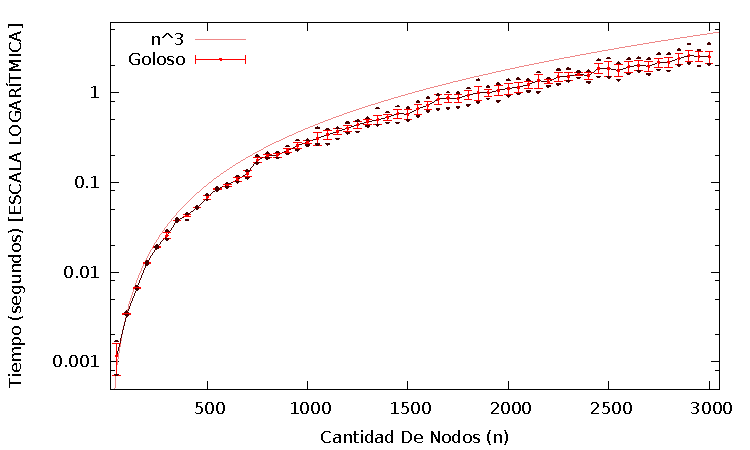
\includegraphics[scale=1.3]{imgs/goloso_3000_50_10.pdf}
\end{center}

\par{Cada punto $\bullet$ en el gráfico representa el promedio de los tiempos
medidos para cada una de las 10 ejecuciones de una determinada cantidad de nodos
del grafo. El tamaño del segmento vertical sobre cada punto $\bullet$ representa
su varianza asociada. Además, para cada cantidad de nodos $n$ se graficaron la
máxima medición con $\blacktriangle$ y la mínima medición con
$\blacktriangledown$.}\\

\par{La función graficada con una curva sin puntos es una función cúbica. Al
estar utilizando escala logarítmica en el eje de ordenadas, esta curva
se ve cóncava. Como se puede observar, la curva definida por la heurística
(la curva resultante de unir los puntos $\bullet$) se asemeja mucho a tal
curva.}

\subsubsection{Optimalidad}

\par{El archivo $opt\_goloso.cpp$ en la carpeta $codigo/goloso$ contiene la
implementación del código que mide el índice de optimalidad de la heurística
golosa. Se ejecutó este programa con $N$ = 100\footnote{Para el test
de performance ejecutamos instancias de tamaño 3000. Sin embargo, para calcular
la optimalidad de la heurísica también debemos ejecutar el algoritmo exacto
con cada instancia, lo que nos restringe el máximo tamaño de entrada.},
$s$ = 1 y $k$ = 10. Es decir, para cada $n$ entero entre 1 y 100, se
generaron 10 grafos aleatorios (con la función $generar\_aristas\_aleatorias$).
Para cada instancia generada se corrió la heurística golosa.
En el siguiente gráfico se muestran los resultados obtenidos.}
\newpage
\begin{center}
\textbf{Gráfico de optimalidad de la heurística golosa en función\\de la cantidad
de nodos del grafo}
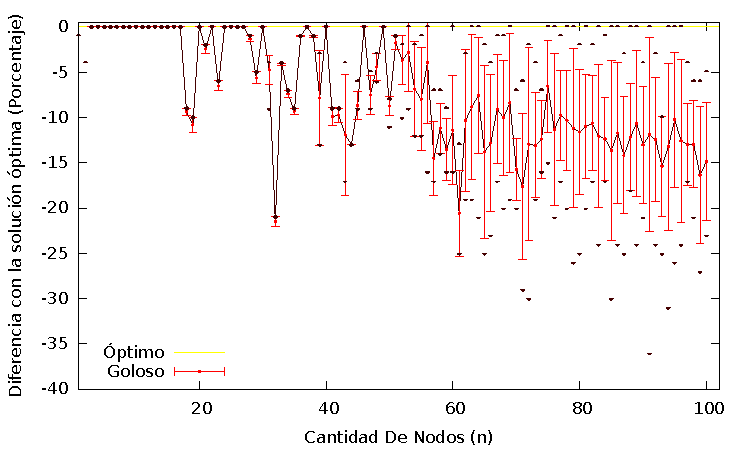
\includegraphics[scale=1.3]{imgs/opt_goloso_100_1_10.pdf}
\end{center}

\par{Cada punto $\bullet$ en el gráfico representa el promedio del índice de
optimalidad para cada una de las 10 ejecuciones de una determinada cantidad de
nodos del grafo. El tamaño del segmento vertical sobre cada punto $\bullet$
representa su varianza asociada. Además, para cada cantidad de nodos $n$ se
graficaron la máxima medición con $\blacktriangle$ y la mínima medición con
$\blacktriangledown$.}\\

\par{La recta $y=0$ representa la solución óptima, así que cuanto más se
asemeje la curva definida por la heurística a dicha recta, mejor es la
heurística. Como se puede observar, para pequeños valores de $n$ la heurística
encuentra siempre, o casi siempre, una solución óptima. Al aumentar la cantidad
de nodos, aumentan tanto la diferencia respecto a la solución óptima, como la
varianza asociada.}\\

\par{Incluso para $n$ mayores, hay instancias para las que la
heurística encuentra una solución óptima. Esto se ve en los $\blacktriangle$
que están sobre la curva $y=0$. Aunque para los mismos $n$ hay instancias en
que la solución devuelta difiere en más del 30\% del óptimo. Como esperábamos,
la varianza en el índice de optimalidad de la heurística es muy grande debido
a que este depende mucho del tipo de grafo que resuelve. Al incrementar la
cantidad de nodos, la curva definida por los resultados del algoritmo
parece estabilizarse. En promedio la heurística golosa parece encontrar
soluciones que representan al rededor del 15\% del óptimo. También parece
no ser peor del 40\%.}\\

\par{Para demostrar que la cota inferior deducida en la sección
\textbf{Comportamiento} es correcta, se realizó otro porgrama que mide el
índice de optimalidad, pero esta vez en lugar de calcular el promedio,
devuelve el valor para cada instancia, además del valor del grado máximo de
cada instancia. El programa está implementado en el archivo $cota\_goloso$ en
la carpeta $codigo/goloso$ y se ejecutó con los mismos parámetros.
En el siguiente gráfico se muestran los resultados obtenidos.}
\newpage
\begin{center}
\textbf{Gráfico de optimalidad de la heurística golosa en función\\de la cantidad
de nodos del grafo (comparación con el grado máximo)}
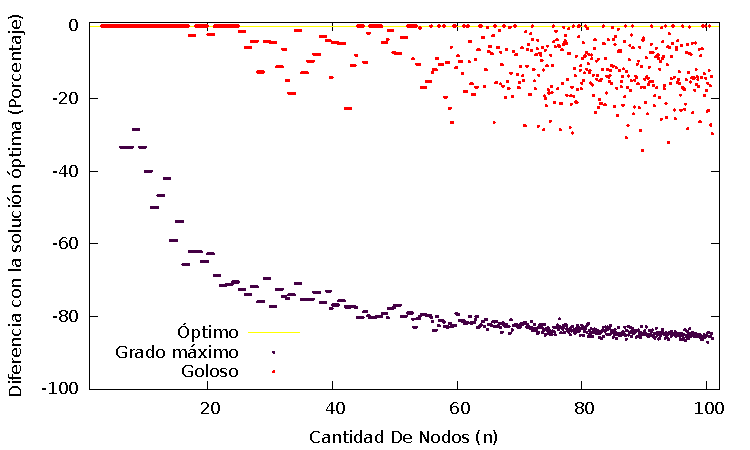
\includegraphics[scale=1.3]{imgs/cota_goloso_100_1_10.pdf}
\end{center}

\par{Cada punto $\bullet$ rojo en el gráfico representa el índice de
optimalidad de una de las 10 instancias de una determinada cantidad de
nodos del grafo. Cada punto $\bullet$ morado representa, para la misma
instancia la diferencia entre el grado máximo del grafo y el valor de una
solución óptima (en procentaje). Para que no se superpongan los puntos
correspondientes a un mismo $n$, la coordenada $x$ de cada punto
no está exactamente sobre $x=n$, sino que está un poco corrido. Como se puede
observar, para cada instancia del problema, el valor de la solución devuelta
por la heurística es mayor o igual al grado máximo del grafo entrada.}
